\chapter{Variational methods in Image Processing}
\label{chapter:variational-methods-in-image-processing}

A track should be constructed to connect some point in space $A$ to a lower altitude point $B$. Which form the track should take if we wish that a ball released at $A$ reaches $B$ in the shortest time? The curve known as brachistochrone or tautochrone is the answer of this puzzle solved by Jean Bernoulli and a classical problem of the \emph{calculus of variations}. 

The main object of calculus of variations are called \emph{functionals} or \emph{energies}, and a simple way to describe it is as a function whose variable is itself a function. Minimizing functionals is a more intricate problem than minimizing an usual function, as the variable in a functional has infinite dimension. Nonetheless, by means of the so called \emph{variations}, one can model infinitely small variations in the functional and do a rigorous analysis of its extremum, the main tool of which is the \emph{Euler-Lagrange} equation.

The calculus of variations found in image processing a fertile field of applications, as images themselves can be seen as functions, and image processing tasks can be modeled as being the results of some functional minimization. In this chapter we present some popular variational techniques to approach image processing tasks, with a particular focus on image segmentation. 

%\startchronology[startyear=1980,stopyear=2020, startdate=false, color=blue!40, stopdate=false, arrow=true, height=3pt]
%\setupchronoevent{textstyle=\tiny,date=false}
%\chronograduation[event]{10}
%\chronoevent[markdepth=20pt]{1984}{\cite{geman84}}\chronoevent[markdepth=-20pt]{1988}{\cite{kass88}}\chronoevent[markdepth=40pt]{1989}{\cite{degiorgi89,mumford89}}\chronoevent[markdepth=-40pt]{1990}{\cite{ambrosio90}}\chronoevent[markdepth=60pt]{1993}{\cite{caselles93}}\chronoevent[markdepth=-60pt]{1994}{\cite{lucy94}}\chronoevent[markdepth=20pt]{1995}{\cite{mcinerney95}}\chronoevent[markdepth=-20pt]{1996}{\cite{kirsch96}}\chronoevent[markdepth=40pt]{1997}{\cite{cohen97,caselles97}}\chronoevent[markdepth=-40pt]{1998}{\cite{bertero98}}\chronoevent[markdepth=60pt]{1999}{\cite{mcinemey99,chambolle99,mcinerney99}}\chronoevent[markdepth=-60pt]{2002}{\cite{vese02}}\chronoevent[markdepth=20pt]{2005}{\cite{stroppa05}}\chronoevent[markdepth=-20pt]{2006}{\cite{chen06}}\chronoevent[markdepth=40pt]{2009}{\cite{benmansour09}}\chronoevent[markdepth=-40pt]{2010}{\cite{peyre10}}\chronoevent[markdepth=60pt]{2011}{\cite{bar11}}\chronoevent[markdepth=-60pt]{2012}{\cite{getreuer12}}\chronoevent[markdepth=20pt]{2015}{\cite{zhdanov15}}\chronoevent[markdepth=-20pt]{2017}{\cite{foare17}}\stopchronology

\section{Inverse problems in imaging}
%In the music world, nothing is as complex as an orchestra score. You have plenty of instruments following different tones, dynamics, intensities, rhythms and so on. But no matter the complexity, given the orchestra score a software can reproduce with perfection the piece of music. It is a totally  different story if you ask it to create the orchestra score from an audio file. Reading the score is a forward problem, and creating the score is an inverse problem.

An archaeological museum decided to digitize some of its collections and make them available for digital visits over the internet. The chosen method of digitization consists into take a set of pictures for each object, in different camera positions, execute a \emph{stereo} algorithm to estimate point depths and finally reconstruct the 3D object. The stereo and reconstruction are examples of \emph{inverse problems} in imaging.

Usually, inverse problems are characterized by a degree of \emph{uncertainty} or \emph{lack of information}. The 2D pictures in the problem above miss depth information, that should be \emph{inferred} by the stereo algorithm. On the other hand, if the shape geometry was known, e.g., the values of mean curvature were known for every infinitesimal point of the shape, then constructing a digital 3D representation would be a \emph{forward problem}. 

We can find examples of inverse problems in several branches of mathematics~\cite{kirsch96}, geophysics~\cite{zhdanov15}, natural language processing~\cite{stroppa05}, astronomy~\cite{lucy94} and the list goes on. The image processing field itself is plenty of them~\cite{bertero98}. In fact, a great part of real world applications consists into inferring parameters of some model, i.e., an inverse problem. In~\cref{ch1:tab:inverse-problems-list} we list some examples of inverse problems and its corresponding forward version.

\begin{table}
\renewcommand{\arraystretch}{1.5}
\footnotesize
\begin{tabular}{|m{7cm}|m{7cm}|}
\hline
\multicolumn{1}{|c|}{\textbf{Inverse problem}} & \multicolumn{1}{c|}{\textbf{Forward problem}} \\
\hline
\textbf{Projection}: Compute vector $v \in \mathbb{R}^3$ whose projection is $P(v) \in \mathbb{R}^2$ & Compute the projection $P(v) \in \mathbb{R}^2$ of vector $v \in R^3$\\
\hline
\textbf{Parameters inference}: Given a set of observations $\Gamma$, infer the parameters $(\mu,\sigma)$ of the Gaussian distribution that describes $\Gamma$ & Given a random variable $X$ following a Gaussian distribution with parameters $(\mu=0,\sigma=1)$, compute the probability $P(X \leq 0.42)$\\
\hline
\textbf{Image denoising}: Given noisy image $\widetilde{\vec{I}}$, compute the original image $\vec{I}$, i.e., the image without noise & Add some random noise to a given image $\vec{I}$ to produce noisy image $\widetilde{\vec{I}}$\\
\hline
\textbf{Image inpainting}: Given image $\widetilde{\vec{I}}$ with a missing patch, reconstruct the removed patch & Remove a patch from image $\vec{I}$ \\
\hline
\textbf{Image segmentation}: Given image $I$, find the labeled partition $\mathcal{I}$ & Given a labeled partition $\mathcal{I}$ of some image $I$, assemble the pieces to create image $I$\\
\hline
\end{tabular}
\caption{Examples of inverse problems and its direct versions. Inverse problems are characterized by uncertainty and parameter inference. }
\label{ch1:tab:inverse-problems-list}
\end{table}

%Predictive text; speech recognition

Another characteristic of inverse problems is that they are usually \emph{ill-posed}. A problem is said to be ill-posed if at least one of the properties below is not respected

\begin{enumerate}
\item{A solution exists and it is unique;}
\item{The solution changes continuously with its parameters}
\end{enumerate}



In order to solve ill-posed problems one should include additional information, i.e., create assumptions over the properties of the sought solution. In the museum problem, for example, one may assume that missing patches of the reconstructed surface should be filled by patches of minimal area. The process of including additional information in ill-posed problems is called \emph{regularization} and its goal is to better condition an ill-posed problem and in the best scenario, transform it into a well-posed one. 

Next, we describe the image model used in this thesis and give a precise definition of the main image problems discussed further on. Examples of such applications can be seen in~\cref{ch1:fig:imaging-problems-real-applications,ch1:fig:imaging-problems-example}.

\subsubsection{Image model}
For matters of simplicity, we limit our discussion to grayscale images, the concepts being mostly extendable to multichannel images. It is convenient to have in mind two different representations of an image.
\begin{center}
\begin{tabular}{rl}
	Discrete: & $\vec{I} \in \mathbb{F}^{m \times n}$ \\
	Continuous: & $f_{\vec{I}}: \Omega \subset \mathbb{R}^2 \rightarrow [0,1]$,
\end{tabular}
\end{center}
%
where $\mathbb{F}$ is a finite set. In this thesis, we define such set as
\begin{align}
	\mathbb{F} &= \{ \frac{i}{255} \; | \; i \in \mathbb{N}, i \leq 255 \}.
\end{align}
%
The discrete representation is interpreted as a sampling of $m \times n$ elements (pixels) of the continuous representation $f_{\vec{I}}$. 

\begin{figure}
\center
\subfloat[$1$ of $2$ aerial images]{
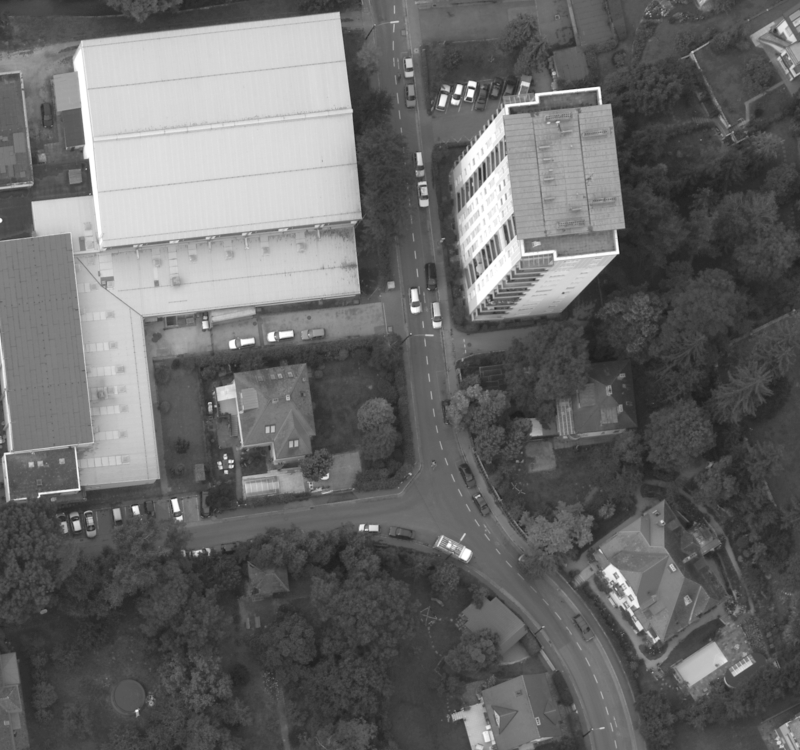
\includegraphics[scale=0.2]{figures/chapter1/applications-gallery/depth-1.png}
}
\subfloat[Depth reconstruction~\cite{pock08}]{
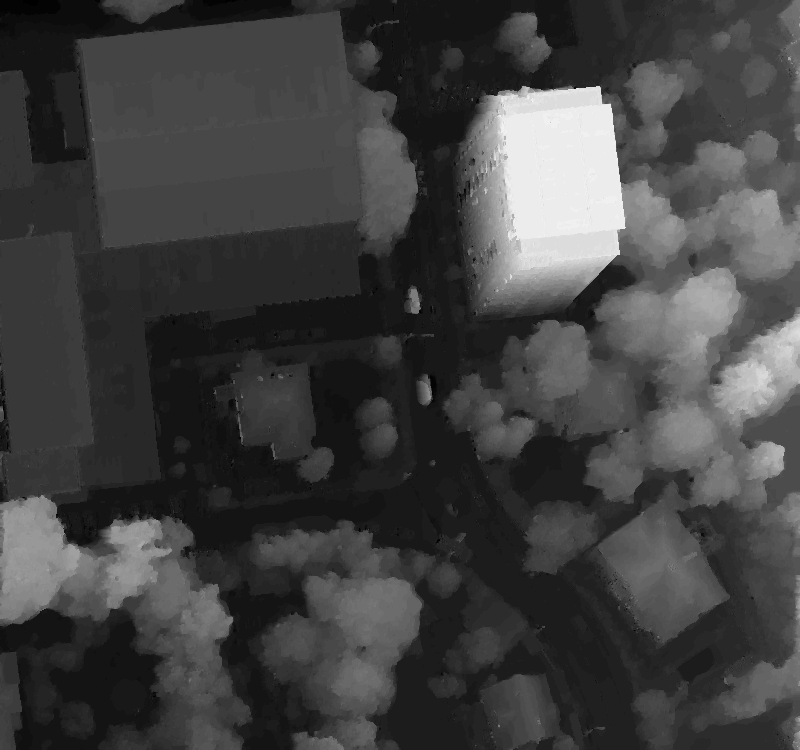
\includegraphics[scale=0.2]{figures/chapter1/applications-gallery/depth-2.png}
}\\
\subfloat[Photo restoration~\cite{masnou98inpainting}]{
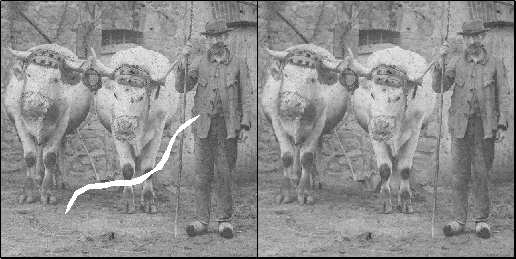
\includegraphics[scale=0.5]{figures/chapter1/applications-gallery/inpainting.png}
}
\subfloat[Vessel segmentation \cite{peyre10,cohen97}.]{
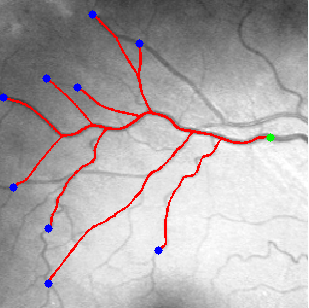
\includegraphics[scale=0.42]{figures/chapter1/applications-gallery/vessel-segmentation.png}
}\\
\subfloat[Input image]{
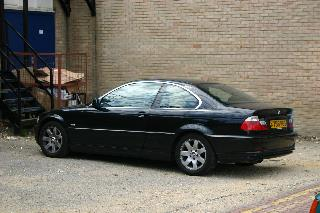
\includegraphics[scale=0.6]{figures/chapter1/applications-gallery/seg-1.png}
}
\subfloat[Multilabel segmentation~\cite{souiai2013co}]{
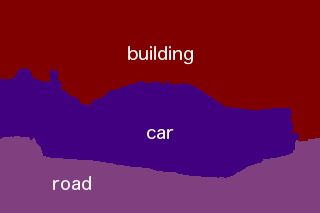
\includegraphics[scale=0.6]{figures/chapter1/applications-gallery/seg-2.png}
}
\caption{\textbf{Real applications of imaging problems}.}
\label{ch1:fig:imaging-problems-real-applications}
\end{figure}

\subsubsection{Image denoising}
Given an image $f_{\vec{\widetilde{I}}}$ corrupted with some noise from an external source, \emph{image denoising} consists in to find an estimation $f_{\widehat{\vec{I}}}$ of the original image that respects some quality criteria, usually encoded by the minimum of a functional $E$. 

Given $f_{\widetilde{\vec{I}}}$, find estimation $f_{\widehat{\vec{I}}}$ such that
\begin{align*}
	f_{\widehat{\vec{I}}} &= \argmin_f E(f,f_{\vec{\widetilde{I}}})
\end{align*}
%
\textbf{Applications:} Restoration of old pictures; enhancement of satellite images.

\subsubsection{Image segmentation}
Given an image $f_{\vec{I}}$, the \emph{image segmentation} problem consists in finding a partition $\mathcal{I}$ of $f_{\vec{I}}$ such that each element of $\mathcal{I}$ is identified with some desired property, usually encoded by the minimum of some functional $E$.
%
%
Given $f_I:\Omega \rightarrow [0,1]$ and a positive integer $n$, find partition $\mathcal{I}^{\star} = \{ \Omega_i \subset \Omega \; | \; i \leq n \}$ such that
\begin{align*}
	\mathcal{I}^{\star} = \argmin_{\mathcal{I}} E(\mathcal{I},f_{\vec{I}}) &\quad  \text{subject to } \begin{array}{l}
	\forall i\neq j:\; \Omega_i \cap \Omega_j = \emptyset\\ 
	\bigcup_i^{n} \Omega_i = \Omega
	\end{array}
\end{align*}
%
\textbf{Applications}: enhance blood vessels in angiograms; track roads in satellite images; identify objects in a scene. 

%In this section we present three paradigms that frequently appear in the literature while coping with variational problems in image processing: Parametric curve evolution (active contours); level-set method (Chan-Vese); and convexification (). All the presented models can be seen as a specification of the classical Mumford-Shah model.


\subsubsection{Image inpainting}
Given an image $f_{\widetilde{\vec{I}}}$ with a collection of missing patches $\mathcal{P}$, \emph{image inpainting} consists in to create an image $f_{\vec{I}}$ with the reconstructed missing patches such that a quality criteria, encoded as the minimum of some functional, is respected

Given $f_{\widetilde{\vec{I}}}$ and missing patches $\mathcal{P}$, find image $f_{\vec{I}}$ such that
\begin{align*}
	f_{\vec{I}} &= \argmin_f E(f,f_{\widetilde{\vec{I}}}) \quad \text{subject to}\; f(\Omega \setminus \mathcal{P}) = f_{\widetilde{\vec{I}}}(\Omega \setminus \mathcal{P}).
\end{align*}
%
\textbf{Applications:} removal of undesired objects in a scene; restoration of old pictures. 

\begin{figure}
\center
\subfloat[Original image]{
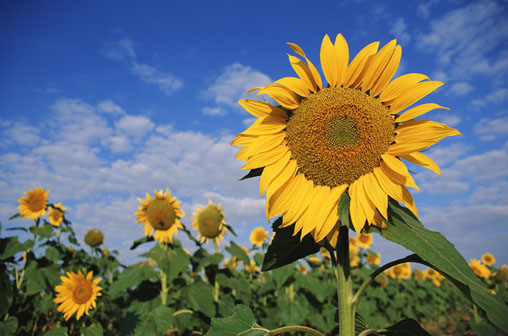
\includegraphics[scale=0.36]{figures/chapter1/inverse-problems/pock-sunflower.png}
}\hspace{2em}%
\subfloat[$10$-partition as in~\cite{chambolle08}]{
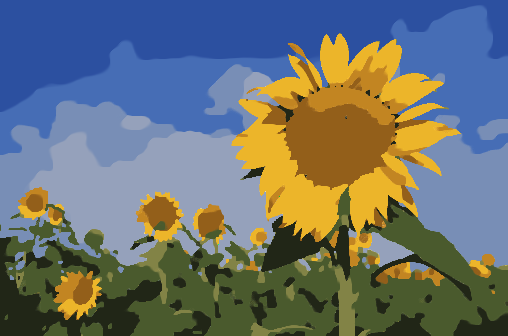
\includegraphics[scale=0.36]{figures/chapter1/inverse-problems/pock-segmentation.png}
}\\%
\subfloat[Noisy image]{
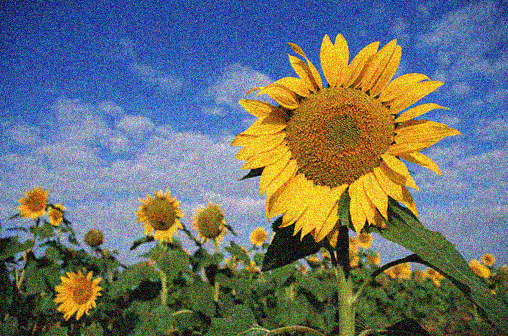
\includegraphics[scale=0.36]{figures/chapter1/inverse-problems/pock-sunflower-noisy.png}
}\hspace{2em}%
\subfloat[Image denoised with FISTA~\cite{beck09a}]{
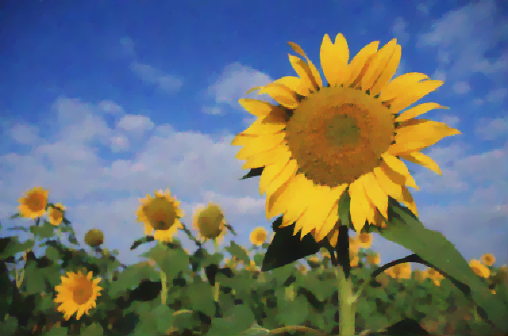
\includegraphics[scale=0.36]{figures/chapter1/inverse-problems/pock-sunflower-fista-denoising-100.png}
}\\%
\subfloat[Inpainting mask]{
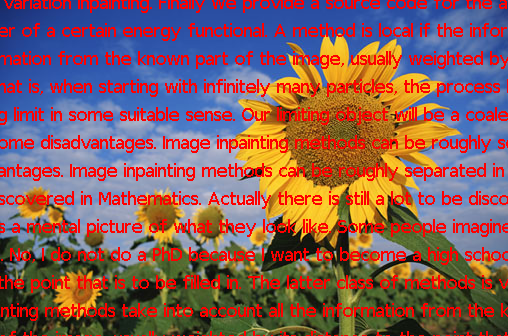
\includegraphics[scale=0.36]{figures/chapter1/inverse-problems/pock-sunflower-mask.png}
}\hspace{2em}%
\subfloat[Inpainted image with~\cite{fedorov15}]{
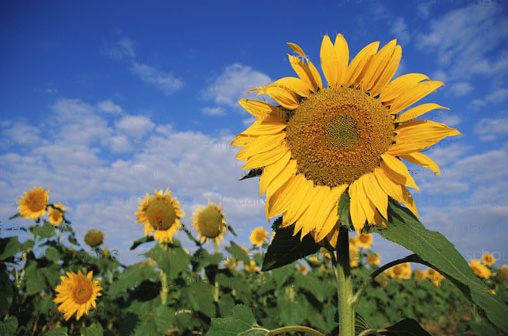
\includegraphics[scale=0.36]{figures/chapter1/inverse-problems/pock-sunflower-inpainted.png}
}%
\caption{\textbf{Imaging problems applications}. From top to bottom row, an example of image segmentation, denoising and inpainting.}
\label{ch1:fig:imaging-problems-example}
\end{figure}


\section{Bayesian rationale and total variation}
\label{ch1:sec:bayesian-rationale}
As remarked in the previous section, inverse problems involve some level of uncertainty about the solution. In order to solve an ill-posed problem we need to regularize it by including additional information, otherwise said, make assumptions.

The maximum a posteriori method was first introduced in the image processing community in the work of~\cite{geman84} and we are going to reproduce here the rational for image denoising. We make two assumptions

\begin{enumerate}
	\item{The noisy image $\vec{\widetilde{I}}$ was obtained by addition of a normal Gaussian noise with $\mu=0,\daniel{\sigma=\lambda^{-1/2}}$ $\daniel{(\lambda>0)}$ to the original image, i.e., 
		\begin{assumption}
		\begin{align}
			\vec{\widetilde{I}} &= \vec{I} + \vec{N},
		\label{ch1:denoising-assumption-1}
		\end{align} 
		\end{assumption}
where $\vec{N}$ is a $(m \times n)$ matrix of random variables $\vec{N}_{i,j}$ and $Pr\big( \vec{N}_{i,j} = n \big) = \frac{1}{\sqrt{2\pi}}\exp(- \daniel{ \lambda } \frac{n^2}{2} )$.		
	}
	\item{Given some function $\rho$, a candidate image estimation $\vec{C}$ has probability	
	\begin{assumption}
	\begin{align}
		Pr(\vec{C}) = \exp(-\rho(\vec{C})).
		\label{ch1:denoising-assumption-2}
	\end{align}	 
	\end{assumption}
	}
\end{enumerate}

%If we want to be precise, the sum operator in~\cref{ch1:denoising-assumption-1} should be redefined to be a closed operator in $\mathbb{F}^{m \times n}$. We skip this definition by arguing that because of the symmetry of the Gaussian distribution the computation of the probabilities that follows remains the same.

 We estimate the unknown original image $\vec{I}$ as the image $\vec{\widehat{I}}$ that is more likely to occur. Applying Bayes' theorem we obtain
\begin{align}
	\vec{\widehat{I}} & = \argmax _{\vec{C}}{Pr(\vec{C} \; | \;\vec{\widetilde{I}})} = \argmax _{\vec{C}} \frac{Pr(\vec{\widetilde{I}} \; | \; \vec{C})Pr(\vec{C})}{Pr(\vec{\widetilde{I}})}.
	\label{ch1:eq:probability-maximization}
\end{align}
%
We have already all the elements to expand~\cref{ch1:eq:probability-maximization}. The probability of having the corrupted image $\vec{\widetilde{I}}$ given a candidate image $\vec{C}$ is derived from~\cref{ch1:denoising-assumption-1}, i.e.,
\begin{align}
	Pr(\vec{\widetilde{I}} \; | \; \vec{C}) &= Pr( \vec{N} = \vec{\widetilde{I}} - \vec{C} ) = \frac{1}{\sqrt{2\pi}}\exp\Big(- \frac{ \daniel{ \lambda }\norm{\vec{\widetilde{I}} - \vec{C} }^2}{2} \Big).
	\label{ch1:eq:probability-corrupted-image-given-original}
\end{align}
%
The denominator term is computed as the joint probability
\begin{align}
	Pr(\widetilde{\vec{I}}) &= \sum_{\vec{J} \in \mathbb{F}^{m \times n}}{Pr(\vec{\widetilde{I}}\;|\; \vec{J})Pr(\vec{J})} = \frac{1}{\sqrt{2 \pi}}\sum_{\vec{J} \in \mathbb{F}^{m \times n}}{\exp\bigg(-\frac{\daniel{ \lambda }}{2}\norm{\widetilde{\vec{I}}-\vec{J}}^2 - \rho(\vec{J})}\bigg).
	\label{ch1:eq:joint-probability}
\end{align}
%
Substituting~\cref{ch1:eq:probability-corrupted-image-given-original,ch1:eq:joint-probability} in~\cref{ch1:eq:probability-maximization} we obtain
\begin{align}
	\vec{\widehat{I}} & = \argmax _{\vec{C}} \frac{1}{\sqrt{2\pi}} \frac{\exp\Big(- \frac{\daniel{ \lambda }}{2}\norm{\vec{\widetilde{I}} - \vec{C}}^2 - \rho(\vec{C}) \Big) }{ \sum_{\vec{J} \in \mathbb{F}^{m \times n}}{\exp\bigg(-\frac{\daniel{ \lambda }}{2}\norm{\widetilde{\vec{I}}-\vec{J}}^2 - \rho(\vec{J})}\bigg) }
	\label{ch1:eq:probability-maximization-expanded}
\end{align}
%
Finnaly, solving~\cref{ch1:eq:probability-maximization-expanded} is equivalent to solve
\begin{align}
	\vec{\widehat{I}} &= \argmin _{\vec{C}} \frac{\daniel{ \lambda }}{2}\norm{\vec{\widetilde{I}} - \vec{C}}^2 + \rho(\vec{C}).
	\label{ch1:eq:minimization-form}
\end{align}
%
The first term appears so often in imaging problems that it has a special name: \emph{data fidelity}. In the denoising problem, the data fidelity term appeared as a consequence of the Gaussian noise model assumption. The second term is also a regularization term and it favors images that respect some desirable property for the problem to be solved. Since natural images has a higher spatial dependency, a reasonable guess for $\rho$ would be a function that has lower value for piecewise smooth data, i.e., images composed by closed regions with smooth variations in its interior but possibly strong discontinuities in their boundaries. 


\subsection{Tikhonov regularization}
\label{ch1:subsec:tikhonov-regularization}
The classical way to optimize~\cref{ch1:eq:minimization-form} is to shift it to a continuous setting, analytically derive some optimization properties and then use this properties to solve the problem in a discrete setting. The continuous reformulation of~\cref{ch1:eq:minimization-form} consists in optimizing the energy functional below
\begin{align}
	f_{\vec{\widehat{I}}} &= \argmin_{f} F(f) = \frac{\daniel{ \lambda }}{2} \int_{\Omega}{ \norm{ f_{\vec{\widetilde{I}}} - f}^2dx} + R(f),
	\label{ch1:eq:variational-formulation}
\end{align}
%
where $R$ is a functional derived from the choice of $\rho$. A popular choice for $R$ is to define it as the $L2$ norm of $\nabla f$, also called the \emph{Tikhonov} regularization term.~\cref{ch1:eq:variational-formulation} is rewritten as
\begin{align}
	f_{\vec{\widehat{I}}} &= \argmin_{f} F(f) = \frac{\daniel{ \lambda }}{2} \int_{\Omega}{ \norm{ f_{\vec{\widetilde{I}}} - f}^2dx} + \int_{\Omega}{ \norm{ \nabla f }^2 dx }.
	\label{ch1:tikhonov-formulation}
\end{align}
%
\subsection{Euler-Lagrange equation}

We can establish some necessary optimization conditions for~\cref{ch1:tikhonov-formulation} by deriving its \emph{Euler-Lagrange} equation. Assume that function $g$ minimizes functional $F$, i.e.,
\begin{align*}
	g &= \argmin_{f}{F(f)}.
\end{align*}
%
Further, assume that there exists a function $w$ that agrees with $g$ at the boundary of $f$' domain, i.e., $w(x)=0,\, \forall x \in \partial \Omega$. Define the function $h$ as
\begin{align*}
	h(\epsilon) &= F(g+\epsilon w)
\end{align*}
%
Therefore, $h$ has a minimum at $\epsilon=0$. Thus,
\begin{align*}
	0 = \frac{dh}{\partial \epsilon}_{| \epsilon=0} &= \frac{d}{\partial \epsilon}_{| \epsilon=0} \int_{\Omega}{ \frac{\daniel{ \lambda }}{2}\norm{f_{\vec{\widetilde{I}}} - g - \epsilon w}^2 + \norm{ \nabla (g + \epsilon w) }^2 \daniel{dx}}  \\
	&= _{| \epsilon = 0} \int_{\Omega}{ \daniel{ \lambda }\norm{ f_{\vec{\widetilde{I}}} - g - \epsilon w}\frac{(f_{\vec{\widetilde{I}}} - g - \epsilon w) }{\norm{f_{\vec{\widetilde{I}}} - g - \epsilon w}}w + 2\norm{ \nabla (g + \epsilon w) }\frac{(\nabla g + \epsilon w)}{\norm{ \nabla (g + \epsilon w) }}\nabla w \daniel{dx}} \\
	&= \int_{\Omega}{ \daniel{ \lambda }(f_{\vec{\widetilde{I}}} - g)w + (\nabla g)\nabla w \daniel{dx}}. 	
\end{align*}
%
Applying integration by parts and using the fact that $w(x)=0,\; \forall x \in \partial \Omega$.
\begin{align*}
		0 &= \int_{\Omega}{ \big( \daniel{ \lambda ( f_{\vec{\widetilde{I}}} - g)} - \Delta g \big)w \daniel{dx}}
\end{align*}
%
Since $w$ could be any function, we can write
\begin{align}
	\daniel{ \lambda ( f_{\vec{\widetilde{I}}} - g)} - \Delta g &= 0
	\label{ch1:eq:variational-necessary-condition}
\end{align}
%
%
Therefore, if $g$ is a minimum of~\cref{ch1:eq:variational-formulation}, then it respects the convex~\cref{ch1:eq:variational-necessary-condition}. Hence, given an initial solution $f$, one can execute a descent method (gradient descent, for example) to find its minimum. In practice, ~\cref{ch1:eq:variational-formulation} is discretized using the samplings $\vec{\widehat{I}}, \vec{\widetilde{I}}$ of $f_{\vec{\widehat{I}}},f_{\vec{\widetilde{I}}}$ and a finite differences scheme is defined to estimate the Laplacian $\Delta$.

The Tikhonov term favors images with smooth variations in color, but the smoothness is not restricted to the interior of regions. Thus, Tikhonov tends to obfuscate the discontinuities that will likely be present in the contour of regions and we have the impression that the image is blurred (see~\cref{ch1:fig:denoising-results}). Nonetheless, Tikhonov term is attractive due to its optimization properties.

\begin{figure}
\center
\subfloat{
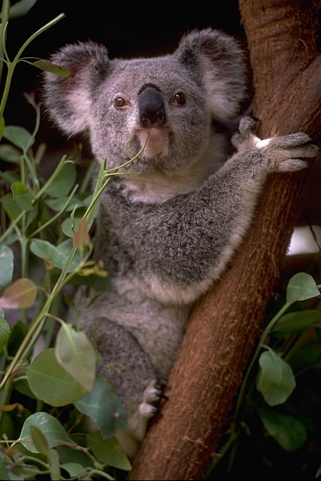
\includegraphics[scale=0.224,valign=t]{figures/chapter1/denoising/coala-original.png}
}\hspace{0.2em} \setcounter{subfigure}{0}
\subfloat[Noisy]{
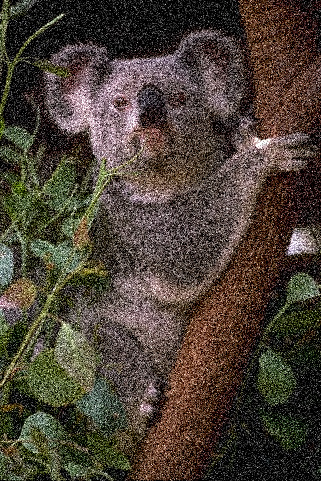
\includegraphics[scale=0.32,valign=t]{figures/chapter1/denoising/coala-noise.png}
}%
\subfloat[Tikhonov]{
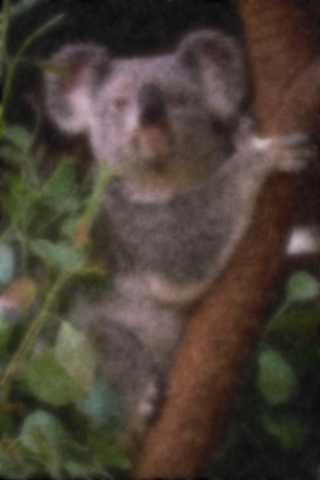
\includegraphics[scale=0.32,valign=t]{figures/chapter1/denoising/coala-tikhonov.png}
}%
\subfloat[Total Variation]{
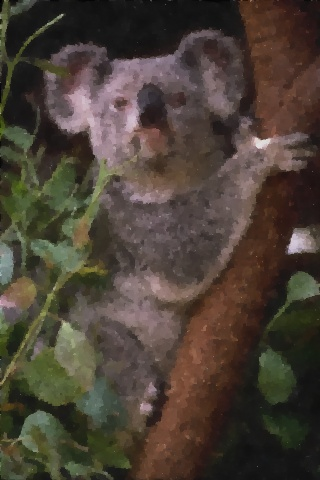
\includegraphics[scale=0.32,valign=t]{figures/chapter1/denoising/coala-rof.png}
}%
\caption{\textbf{Tikhonov x Total variation denoising}. Total variation is capable to better preserve discontinuities across edges than Tikhonov. }
\label{ch1:fig:denoising-results}
\end{figure}


\subsection{Total variation regularization}
An alternative to Tikhonov regularization is to use the so called \emph{total variation} of the image function. For a smooth function $f$, its total variation is computed as
\begin{align*}
	TV(f) &= \int_{\Omega}{ \norm{ \nabla f } }.
\end{align*}
%
For a more general (possibly not differentiable) locally integrable function $f:\Omega \rightarrow \mathbb{R}^n$, its total variation is defined as
\begin{align*}
	TV(f) &= \sup \left\{ \int_{\Omega}{\nabla u \cdot \phi} \; | \; \phi \in C_c^{1}(\Omega, \mathbb{R}^n) \text{ and } \norm{\phi}_{\infty} \leq 1 \right\} \\
		  &= \sup \left\{ - \int_{\Omega}{u \nabla \cdot \phi} \; | \; \phi \in C_c^{1}(\Omega, \mathbb{R}^n) \text{ and } \norm{\phi}_{\infty} \leq 1 \right\},	
\end{align*}
%
where $\phi$ is vector-valued infinitely differentiable function with compact support. The image denoising total variation model is written as
\begin{align}
	f_{\vec{\widehat{I}}} &= \argmin_{f} \frac{\lambda}{2} \int_{\Omega}{ \norm{ f_{\widetilde{I}} - f}^2dx} + TV(f).
	\label{ch1:eq:total-variation-denoising}
\end{align}
%
The ROF model~\cite{rudin92} assumes the image representation is smooth, and from the Euler-Lagrange equation of~\cref{ch1:eq:total-variation-denoising} the following gradient flow is derived:
\begin{align*}
	\frac{\partial f}{\partial t} &= \nabla \cdot \left( \frac{\nabla f}{\norm{ \nabla f} } \right) - \lambda (f_{\widetilde{\vec{I}}} - f)
\end{align*}
%
The left term is not differentiable, and a small $epsilon >0$ is added to the denominator in order to avoid numerical instability. However, the calibration of $\epsilon$ might be delicate, since a small $\epsilon$ might not be sufficient to avoid instability and a larger $\epsilon$ may disfigure the model. In~\cite{chambolle04} the total variation definition is exploited to create a convergent algorithm that works by successive projections and that solves model~\cref{ch1:eq:total-variation-denoising}. In~\cite{beck09a} a modified version of the previous algorithm has proven to have faster convergence. 

The total variation term is characterized by its smooth properties while partially preserving some discontinuities across the edges. In this sense, total variation models produce results with sharper edges than those produced by the Tikhonov term (see~\cref{ch1:fig:denoising-results}) .

\section{Standard techniques}

In this section we give an overview of the key techniques in variational models for problems in image processing. We start by describing the most influential model in this category.

\subsubsection{Mumford-Shah}
The $L2$-norm regularization has nice optimization properties, but it does not preserve discontinuities along the object boundaries. This effect is attenuate using a $L1$-norm, but it it not sufficient to avoid blurred edges. The\emph{Mumford-Shah} functional~\cite{mumford89} handles this issue by incorporating the edges in its formulation in the form of a set of discontinuities $\mathcal{K}$ and limiting the $L2$-norm regularization to points in the interior of objects, i.e.,  $\Omega \setminus \mathcal{K}$. Moreover, the set $\mathcal{K}$ itself is compelled to be of small length. The Mumford-Shah model consists in minimizing the following functional 
\begin{align}
	(f_{\vec{\widehat{I}}},\mathcal{\widehat{K}}) &= \argmin_{f,\mathcal{K}} \alpha \int_{\Omega}{ \norm{f_{\vec{\widetilde{I}}}-f}dx} + \beta \int_{\Omega \setminus \mathcal{K}}{\norm{\nabla f}dx} + \lambda Per(\mathcal{K})
	\label{ch1:mumford-shah-functional}
\end{align}
%
The functional can be seen as a model for both denoising and segmentation problems. The function $f_{\vec{\widehat{I}}}$ being the denoising solution and $\mathcal{\widehat{K}}$ the segmentation solution.~\cref{ch1:mumford-shah-functional} is proven to have a minimizer~\cite{degiorgi89}, and in the case $\mathcal{K}$ is fixed, the minimizer is unique (see chapter 25 of~\cite{bar11}). However, to find a minimizer of~\cref{ch1:mumford-shah-functional} is a challenging task due to its non-convexity.

Nonetheless, there exist several approximations to the Mumford-Shah functional. We refer to the phase-field model of~\cite{ambrosio90}; the finite-differences scheme of~\cite{chambolle99}; the level-set method of~\cite{vese02}; the convex relaxations of~\cite{pock09,strekalovskiy14}; and the discrete calculus approach of~\cite{foare17}.

\subsection{Curve evolution}

\subsubsection{Active contours}
\emph{Active contours} or snakes is a supervised method for doing image segmentation. In the original work~\cite{kass88}, an initial parametric curve $C_0(q) \rightarrow (x(q),y(q))$ is evolved towards the local minimum of the snakes energy
\begin{align}
	F(C) &= \alpha Length(C) + \beta Smoothness(C) + \gamma Edge(C) \nonumber \\
	F(C) &= \alpha \int_{0}^{1}{ \bignorm{ \frac{dC}{\partial q} }^2 dq } + \beta \int_{0}^{1}{ \bignorm{ \frac{d^2C}{\partial q^2} }^2dq} -\gamma \int_{0}^{1}{ \norm{ \nabla f_I(C(q))}^2 dq}
	\label{ch1:eq:snakes-energy}
\end{align}
%
The length and smoothness regularization term favors curves of smooth variations and  small length while the edge term compels the curve to stop at regions of high variation of color intensity. 

The snakes method was devised having an interactive framework in mind. First of all, the user must set the initial curve close to the object to be segmented, and besides that, a set of additional tools as anchor points, repulsion and spring forces are available for online modification of the problem. The user can make use of these tools to conveniently perturb the current solution and force the curve to evolve to the expected local optimum.

The active contours is an influential paradigm for image segmentation and it was particularly popular for segmenting medical images~\cite{mcinerney99}. Variations of the original model include extension to 3D-segmentation~\cite{mcinemey99} and topologically adaptable snakes~\cite{mcinerney95}.

Some drawbacks in the active contours formulation include its non-intrinsic definition, i.e., the curve is not defined in terms of its geometric properties and its representation depends on the chosen parametrization; and, partially as consequence of the latter, its inability to change the initial curve topology. One needs to initialize several snakes in order to correctly segment a picture with several holes, for example. 

%This approach is also non-
%intrinsic, since the energy depends on the parametriza-
%tion of the curve and is not directly related to the objects
%geometry. As we show in this paper, a kind of “re-
%interpretation” of this model solves these problems.
%See for example (Malladi et al., 1995) for comments
%on other advantages and disadvantages of energy ap-
%proaches of deforming contours, as well as an extended
%literature on snakes.

%Energy minimization x Curve evolution approaches

%In this paper a particular case of the classical en-
%ergy snakes model is proved to be equivalent to find-
%ing a geodesic curve in a Riemannian space with a
%metric derived from the image content. This means
%that in a certain framework, boundary detection can
%be considered equivalent to finding a curve of mini-
%mal weighted length. This interpretation gives a new
%approach for boundary detection via active contours,
%based on geodesic or local minimal distance computa-
%tions.
 
%O modelo do Caselles jah era um modelo do tipo level set
%que ja era capaz de surmontar os obstaculos de uma evolucao
%sem alteracao de topologia, como eh o caso das snakes. 
 
%Solving the problem of
%snakes amounts to finding, for a given set of constants
%α, β, and λ, the curve C that minimizes E. Note that
%when considering more than one object in the image,
%for instance for an initial prediction of C surrounding
%all of them, it is not possible to detect all the objects.
%Special topology-handling procedures must be added.
%Actually, the solution without those special procedures
%will be in most cases a curve which approaches a con-
%vex hull type figure of the objects in the image. In
%other words, the classical (energy) approach of snakes
%can not directly deal with changes in topology.


%This will allow to achieve
%smooth curves in the proposed approach without hav-
%ing the high order smoothness given by β 6= 0 in
%energy-based approaches. 3 Moreover, the second order
%smoothness component in (1), assuming an arc-length
%parametrization, appears in order to minimize the to-
%tal squared curvature (curve known as “elastica”). It is
%easy to prove that the curvature flow used in the new ap-
%proach and presented below decreases the total curva-
%ture (Angenent, 1991). The use of the curvature driven
%curve motions as smoothing term was proved to be very
%efficient in previous literature (Alvarez et al., 1993;
%Caselles et al., 1993; Kimia, —; Niessen et al., 1993;
%Malladi et al., 1994, 1995, —; Sapiro and Tannenbaum,
%1993), and is also supported by our experiments in Sec-
%tion 4. Therefore, curve smoothing will be obtained
%also with β = 0, having only the first regularization
%term. Assuming this (1) reduces to


%Leaving \beta \neq 0 in the active contours lead to a fourth-order
% term in the Euler-Lagrange equation

%The functional in (2) is not intrinsic since it depends
%on the parametrization q that until now is arbitrary.
%This is an undesirable property, since parametrizations
%are not related to the geometry of the curve (or object
%boundary),

%The Euclidean heat flow, what I call the curvature flow,
%
%is well known for
%its very satisfactory geometric smoothing properties
%(Angenent, 1991; Gage and Hamilton, 1986; Grayson,
%1987). (It was extended in (Sapiro and Tannenbaum,
%1993a, b, 1994) for the affine group and in (Olver
%et al., 1994, —; Sapiro and Tannenbaum, 1993) for
%others.) The flow decreases the total curvature as well
%as the number of zero-crossings and the value of max-
%ima/minima curvature.

%It is a shortening and smoothing terms simultaneously.


%This is achieved with the help of the
%mentioned level-set numerical algorithm for curve evo-
%lution, developed in (Osher and Sethian, 1988; Sethian,
%1989) and already used by others for different im-
%age analysis problems (Chopp, 1991; Kimia et al., —;
%Kimmel et al., 1995, —; Kimmel and Sapiro, 1995;
%Sapiro et al., 1993; Sapiro and Tannenbaum, 1993a,
%1995). In this case, the topology changes are automat-
%ically handled without the necessity to add specific
%monitoring on the deforming curve or any heuristic
%criterion.

%This energy is however not intrinsic to the curve geometry, since it
%also depends on the parameterization of the curve. This is why these
%two terms were replaced by length element and curvature to obtain an
%intrinsic energy and define a geometric model [57]. Since it is complex
%to deal with the curvature term, it was removed in that model, as
%well as in the level set approach of Malladi et al. [179]


%The unsigned distance function φ̃ s is the unique
%viscosity solution of the Eikonal equation
%||∇ φ̃ t (x)|| = 1
%and ∀ s ∈ [0, 1], φ̃ t (γ(s)) = 0.
%(3.9)
%This equation can be solved in O(N log(N )) operations on a regular
%grid of N pixels using the Fast Marching algorithm detailed in Section
%2.3

%In the case of noisy images, the initial image is convolved with a Gaussian kernel

%Fethallah Benmansour and Laurent D. Cohen. Fast object segmentation by
%growing minimal paths from a single point on 2D or 3D images. J. Math.
%Imaging Vis., 33(2):209–221, February 2009.

%Vessel segmentation using shortest paths. Top left: original retinal image from
%DRIVE database [199].


%Relation with watershed. If the geodesic distance map U S is ap-
%proximated with morphological operators, as detailed in Section 2.8.1,
%the Voronoi segmentation corresponds to the result of the water-
%shed algorithm initially proposed in [28] and extended for instance
%in [283, 198, 188]. For the watershed algorithm, the set of initial points
%S is usually chosen as the local minima of the map W (x), possibly after
%some smoothing pre-processing.

\subsubsection{Geometric active contours}
Parametric models as snakes are often criticized because of their non-intrinsic definition, i.e., the energy is not defined in terms of the geometric properties of the contours. That makes the theoretical analysis of the snakes model harder, as the evolution of the contour itself depends of the chosen parametrization. In~\cite{caselles93} the authors propose a model based on the mean curvature motion of the level-sets of a $C^2$ function $u$.


Let $u:\Omega \subset \mathbb{R}^2 \rightarrow [0,1]$ be a $C^2$ function. The curvature at its $k$-th level set is given by
\begin{align*}
	\kappa (x,y) &= \nabla \cdot \left( \frac{\nabla u}{\norm{\nabla u}} \right), \quad \forall (x,y) \in \left\{ \; (x,y) \; | \; u(x,y)=k \; \right\}
\end{align*}
%
%
The \emph{geometric active contour} model consists into evolving an extension of $u$, by including an artificial time parameter $t$, and compute the steady solution of the flow
\begin{align}
	u(0,x,y) &= u(x,y) \nonumber \\
	\frac{du}{dt} &= g( \norm{\nabla f_{\vec{I}}} )\norm{\nabla u}\nabla \cdot \left( \frac{\nabla u}{\norm{\nabla u}}  + v \right),
	\label{ch1:geometric-active-contour}
\end{align}
%
where $g$ is a non-increasing function that plays the role of an edge-detector, e.g., $g(x) = 1/(1+x)^2$. The function $u$ can be initially defined as a smoothed version of $1 - \chi_C$, where $\chi_C$ is the characteristic function of some set $C \in \Omega $ that contains the objects to be segmented. 

Following~\cref{ch1:geometric-active-contour}, the gray level at some point $(x,y)$ changes proportionally to the curvature of its belonging level set. The constant $v$ forces the change in $u$ to be always positive, i.e., pixels gets lighter, never darker. The term $\norm{\nabla u}$ allows $u$ to evolve only at some neighborhood of the $0$-level-set boundary and the term $g(\norm{\nabla f_{\vec{I}}})$ makes the evolution to stop if an edge is reached. At the steady solution of~\cref{ch1:geometric-active-contour} the segmented objects of $\vec{I}$ corresponds to the $0$-level set of $u$.

Differently from the snakes, the geometric active contours handle changes in topology of the initial curve. In figure~\cref{ch1:fig:comparison-curve-evolution}, the initial $0$-level set of $u$ splits in three disjoint sets at the steady solution of~\cref{ch1:geometric-active-contour}. However, the geometric active contour models cannot segment objects with holes without including a region-based term~\cite{chen06}.

\begin{figure}
\center
\subfloat[Active contours]{
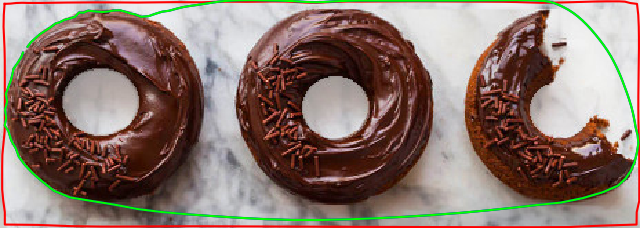
\includegraphics[scale=0.5]{figures/chapter1/segmentation/active-contour-don.png}
}\hspace{2em}%
\subfloat[Geometric active contours]{
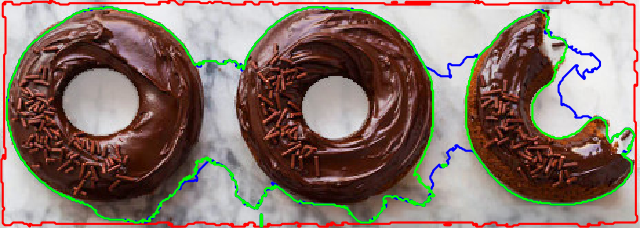
\includegraphics[scale=0.5]{figures/chapter1/segmentation/geodesic-seg-don.png}
}\hspace{2em}%
\subfloat[Chan-Vese]{
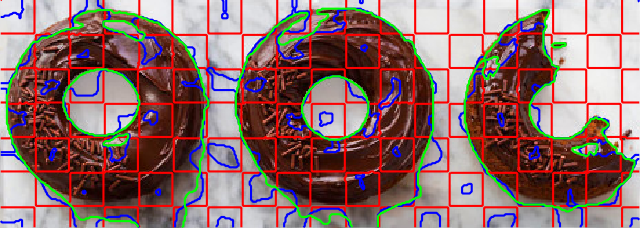
\includegraphics[scale=0.5]{figures/chapter1/segmentation/chan-vese-seg-don.png}
}%
\caption{\textbf{Curve evolution models}. Segmentation results of three curve evolution models. From top row to bottom: active contours, geometric active contours and Chan-Vese. The initial curve ($0$-level set) is colored in red and the final one is colored in green.}
\label{ch1:fig:comparison-curve-evolution}
\end{figure}


\subsection{Level set}
	The active contour and its geometric version are both edge-based methods, a natural strategy for image segmentation but with limitations, e.g., the models may encounter some difficulties to segment objects with holes. The \emph{Chan-Vese} method proposes the inclusion of a region-based term and it generalizes the level-set approach already presented in the geometric active contour model. 
	
	Let $f_{\vec{I}}:\Omega \subset \mathbb{R}^2 \rightarrow \mathbb{U}^2$ a grayscale image and $F \subset \Omega$ an open set such that the pair $(F,\Omega \setminus F)$ is the searched binary partition. Further, assume that there exists a function $\phi: \Omega \rightarrow \mathbb{R}$ with bounded first derivative. The image partitions are identified in the following fashion
\begin{align*}
	\phi(x) < 0,&\quad \forall x \in F \\
	\phi(x) = 0,&\quad \forall x \in \partial F\\
	\phi(x) > 0,&\quad \forall x \in \Omega \setminus \overline{F}
\end{align*}
%	
	In possession of the partition descriptor $\phi$, the following energy is proposed	
\begin{align}
	F(\phi,x) &= \mu Length(\phi,x) + \nu Area(\phi,x) + \lambda_1 Foreground(\phi,x) + \lambda_2 Background(\phi,x) \nonumber \\	
	&= \mu \int_{\Omega}{\delta_0(\phi(x))\norm{ \nabla \phi(x)}dx} + \nu \int_{\Omega}{H(\phi(x))dx} \nonumber \\
	&+ \lambda_1 \int_{\Omega}{\big(1-H(\phi(x))\big)\norm{f_{\vec{I}}(x) - c_F}^2dx} + \lambda_2\int_{\Omega}{H(\phi(x)\norm{f_{\vec{I}}(x)-c_B}^2dx},
	\label{ch1:eq:chan-vese-functional}
\end{align}
%
where $H(x)$ is the Heaviside function and $\delta_0$ the standard Dirac delta function, i.e.,
\begin{align*}
\begin{array}{ll}
	H(x) = \left\{ \begin{array}{ll}
		1, & x \geq 0 \\
		0, & \text{otherwise},
	\end{array}\right. & \quad 
	\delta_0( x ) = \left\{ \begin{array}{ll}
								+ \infty,& x=0\\
								0,& \text{otherwise}.
							\end{array}\right. \text{ and } \int_{-\infty}^{+\infty}{\delta_0(x)dx}=1.
\end{array}
\end{align*}
%
The parameters $c_f,c_b$ are defined as the average color intensity in the interior of the foreground and background regions, respectively
\begin{align*}
\begin{array}{ll}
	\displaystyle c_F = \frac{\int_{\Omega}{\big(1-H(\phi(x))\big)f_{\vec{I}}(x)dx}}{\int_{\Omega}{\big(1-H(\phi(x))\big)dx}}, & 	
	\displaystyle c_B = \frac{\int_{\Omega}{H(\phi(x))f_{\vec{I}}(x)dx}}{\int_{\Omega}{H(\phi(x))dx}}.
\end{array}
\end{align*}
%
Next, the Euler-Lagrange equation of~\cref{ch1:eq:chan-vese-functional} is calculated and used to define a gradient flow to minimize~\cref{ch1:eq:chan-vese-functional}, in a similar fashion as done in~\cref{ch1:subsec:tikhonov-regularization}. In order to be numerically tractable, the Heaviside and Dirac delta function are regularized as 
\begin{align*}
\begin{array}{ll}
	\begin{array}{ll}
		\displaystyle H_{\epsilon}(x) &= \displaystyle \frac{1}{2}\left( 1 + \frac{2}{\pi}\arctan(\frac{x}{\epsilon}) \right),
	\end{array} & 	
	\begin{array}{ll}
		\displaystyle \delta_{\epsilon}(x) &= \displaystyle \frac{\epsilon}{\pi(\epsilon^2 + x^2)}.
	\end{array}	
\end{array}
\end{align*}

The initial level set function can be set as any function with bounded first derivative, but it is recommended to use the checkerboard function $\phi=\sin(\pi/5 x_1)\sin(\pi/5x_2)$ which is reported~\cite{getreuer12} to have fast convergence. In~\cite{vese02}, the Chan-Vese authors extended their method to contemplate colored images and multisegmentation. An illustration is presented in~\cref{ch1:fig:comparison-curve-evolution}


%Relation with the minimal partition problem, whose solution existence has been proven, and piecewise constant MS  


\subsection{Minimum path}

In a sequel work, the authors of geometric active contours established a link between their geometric model in~\cite{caselles93} and the computation of geodesics in a regular surface~\cite{caselles97}. 

The length of a parametric curve $C(q)$ according to an isotropic metric of potential $W(C)$ is calculated as 
\begin{align}
	L(C) &= \int{W(C)\norm{C_q} dq}.
	\label{ch1:eq:length-isotropic-metric}
\end{align}
%
~\cref{ch1:eq:length-isotropic-metric} is used to compute shortest paths between two points according to the given metric. By properly setting the potential $W$, we can make object boundaries in an image $f_{\vec{I}}$ to match the curves of shortest length, for example, letting $W=g(\norm{\nabla f_I})$ as in~\cref{ch1:geometric-active-contour} we obtain
\begin{align}
	L(C) &= \int{g\big(\norm{\nabla f_I(C(q))}\big)\norm{C_q} dq}.
	\label{ch1:eq:geodesic-energy}
\end{align}
%
In~\cite{caselles97} the authors show that the snakes model without the smoothness term($\beta=0$) is equivalent to geodesics computations, the metric changing accordingly with the models parameters. The isotropic metric above is equivalent to the case in which the length and image terms of the snakes model are equal.

Given an initial curve $C_0(q)$, a local minimizer for~\cref{ch1:eq:geodesic-energy} can be computed by finding the steady solution of the following flow derived from its Euler-Lagrange equation
\begin{align}
	C(0,q) &= C_0(q)\\
	\frac{dC}{dt} &= (g\kappa - \nabla g \cdot \vec{n})\vec{n},
	\label{ch1:eq:curve-evolution}
\end{align}
%
where $\vec{n}$ is the normal vector to the curve $C$ at $(t,q)$. One can show that, given an initial function $u \in \mathcal{C}^2$ such that $u$ is negative (positive) in the interior (exterior) of its $0$-level set, the solution of~\cref{ch1:eq:curve-evolution} equals the steady solution of
\begin{align}
	u(0,x,y) &= u_0(x,y) \\
	\frac{du}{dt} &= g\norm{\nabla u}\kappa + \nabla g \cdot \nabla u
	\label{ch1:eq:surface-evolution}
\end{align}
%
Comparing~\cref{ch1:eq:surface-evolution} with~\cref{ch1:geometric-active-contour} we notice that the $\nabla g \cdot y$ term was included while the $v$ parameter was removed. The geometric active contour stops as soon as an ideal edge is found (a threshold should be set), which is particularly bad for real images segmentation, as it is likely that the flow will stop at the first variation of color intensity. The new term allows the flow to evolve even in those cases. Nonetheless, one can include again the $v$ parameter, as it permits to increase the convergence in some cases.

The relation between segmentation and geodesic computation inspired several works. Elongated and thin objects as blood vessels or roads in satellite images are the global optimum of a geodesic computation in which the minimum path is constrained to lie between two points~\cite{cohen97}. Further development of this work reduced the initialization to just a single point~\cite{benmansour09}. Anisotropic metrics aligned to the image edges are reported to return improved solutions for blood vessels segmentation~\cite{jbabdi08,benmansour11}. Ideas from Chan-Vese and Geodesic models are put together in~\cite{chen06}. Finally, an elucidating review of geodesic methods in computer vision can be found in~\cite{peyre10}.

\subsection{Convex relaxation}

A set $\Omega$ is convex if for all $a,b \in \Omega$, every element in the line connecting $a,b$ also lie in $\Omega$. A function $f:\Omega \rightarrow \mathbb{R}$  is convex if its domain $\Omega$ is convex and the following inequality holds
\begin{align*}
	f(\alpha x + (1-\alpha)y) \leq \alpha f(x) + (1-\alpha)f(y).
\end{align*}
%
Convexity is a desirable property in optimization problems because any local minimizer (maximizer) is also a global one. In other words, methods that optimizes $f$ do not depend on its initialization. Therefore, it is of great interest to find convex formulations for image processing problems.

Ideally, one would look for the so called convex envelope of $f$, which is the tightest convex function $\widetilde{f}$ such that $\widetilde{f} \leq f$. In fact, one can compute the envelope of a function $f$ by taking its convex biconjugate.
%
\begin{definition}{Convex conjugate}
	Let $f:\Omega \rightarrow \mathbb{R} \cup \{ +\infty, -\infty\}$. Its convex conjugate is defined as
	\begin{align*}
		f^{*}(y) &= \sup_x y^{T}x - f(x)
	\end{align*}
\end{definition}
%
The biconjugate $f^{\star \star}$ is the convex envelope of $f$. In fact, if $f$ is convex and lower-semicontinuous, $f^{\star \star}=f$ (Frenchel's inequality). Unfortunately, the computation of the biconjugate is known only for a few functions. Nonetheless, the conjugate is key to prove properties on convex optimization algorithms as those based on the proximal operator~\cite{chambolle04,beck09a}. 


In order to use tools from convex optimization one needs to define a convex energy. Very often in imaging problems the functionals are defined over a non-convex function space, for example, in the binary denoising or the multilabeling problem, in which the optimization function has a discrete range. A straightforward approach is to simply relax the range to a continuous set and execute a standard optimization method. The discrete solution is then obtained by simple rounding. However, fewer are the cases in which the projected solution is optimum or even meaningful to the original problem. A technique that gives guarantees with respect to the quality of the back projected solution is \emph{functional lifting}.

\subsubsection{Functional lifting}

Consider the binary image denoising problem. Let $f_{\widetilde{\vec{I}}}$ the observed noisy image and consider the total variation model for binary denoising
\begin{align}
	\min_{f_{\vec{I}}:\Omega \rightarrow \{0,1\} } E^{2-den}(f_{\vec{I}}) &= \min_{f_{\vec{I}}} \int_{\Omega}{\norm{\nabla f_{\vec{I}}}} + \lambda \int_{\Omega}{ (f_{\vec{I}}-f_{\widetilde{\vec{I}}})^2}
	\label{ch1:eq:binary-denoising-model},
\end{align}
%
This model is not convex, as the optimization  variable $f_{\vec{I}}$ belongs to the non-convex domain of binary functions. The corresponding level-set formulation of~\cref{ch1:eq:binary-denoising-model} (in the same spirit of the Chan-Vese model) is given by
\begin{align}
	\min_{}{ \int_{\Omega}{ \norm{\nabla H(\phi(x))} } + \lambda \int_{\Omega}{\left( H(\phi(x)) - f_{\widetilde{\vec{I}}}(x) \right)^2}}.
	\label{ch1:eq:2-den-level-set-energy}
\end{align}
%
Whose a local minimum is a steady solution of
\begin{align}
	\frac{d\phi}{dt} &= H_{\epsilon}^{\prime}(\phi)\left(  \nabla \cdot \left( \frac{ \nabla \phi}{\norm{\nabla \phi}}\right) + 2\lambda(f_{\widetilde{\vec{I}}}(x) - H_{\epsilon}(\phi)) \right)
	\label{ch1:eq:level-set-ball-flow}
\end{align}
%
We reproduce the example given in~\cite{chan06} to illustrate a situation in which the Chan-Vese method returns a local optimum solution. Assume that the observed image is the characteristic function of a ball of radius $R$, i.e., $f_{\widetilde{\vec{I}}}(x) = \mathbf{1}_{B_R}(x)$. Moreover, we set the initial guess of the level-set function to be precisely the observed image, i.e., $\phi_0(x) = f_{\widetilde{\vec{I}}}(x)$. The evolution given by~\cref{ch1:eq:level-set-ball-flow} maintains the radial symmetry of $\phi_0$, which means that $\phi^{(t)}$ will represent the characteristic function of some ball of radius $r$. In other words, for this particular setting, ~\cref{ch1:eq:2-den-level-set-energy} is equivalent to
\begin{align}
	\min_{r} g(r,\lambda) &= \min_r 2\pi r + \lambda \pi |R^2-r^2|, \quad r \geq 0.
	\label{ch1:eq:balls-evolution}
\end{align}
%
%
~\cref{ch1:eq:balls-evolution} has a local minimum at $r=R$ and a local maximum at $r=1/\lambda$. Depending on the value of $\lambda$, its global minimizer will be at $r=0$ or $r=R$. For a fixed $\lambda$, let's consider the case in which $g(0,\lambda) < g(R,\lambda)$.
\begin{align*}
	g(0,\lambda) &\leq g(R,\lambda) \\
	\lambda \pi R^2 &\leq 2\pi R \\
	R &\leq \frac{2}{\lambda}
\end{align*}
%
Therefore, for $R \in (1/\lambda, 2/\lambda)$, the flow of~\cref{ch1:eq:level-set-ball-flow} is going to stop at the local minimum $r=R$, even the global minimum being located at $r=0$. 
%
The parameter $\lambda$ is set by the user to calibrate the denoise capabilities of the model. In the example of~\cref{ch1:fig:local-solution-level-set}, it indicates whether a ball of certain radius should be considered as an object or as a noise element. In the illustrated case, with $\lambda=1$, the optimal solution consists to segment only the ball of largest radius in the picture, but Chan-Vese fails to converge to this solution.

\begin{figure}
\center
\subfloat[Input image and contour of lowest energy for $\lambda=1$]{
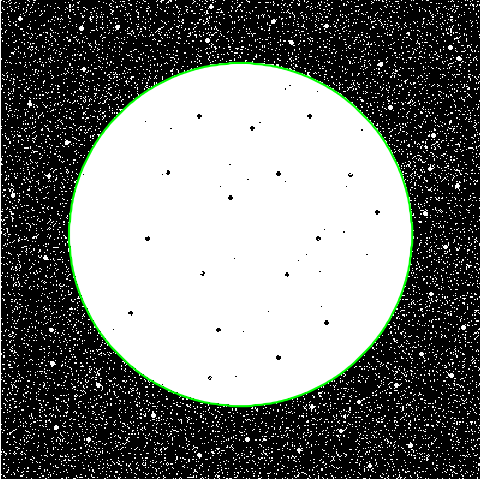
\includegraphics[scale=0.5]{figures/chapter1/convex/reference_contour.png}
}\hspace{3em}%
\subfloat[Result of level-set method for $\lambda=1$]{
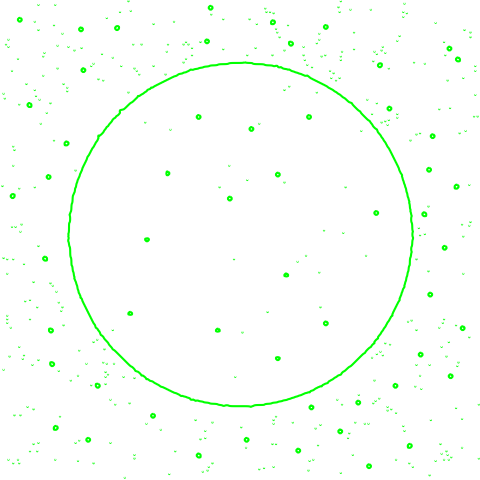
\includegraphics[scale=0.5]{figures/chapter1/convex/lbda_1.png}
}%
\caption{\textbf{Level-sets return local optimum solutions.} Level-set result of~\cref{ch1:eq:binary-denoising-model} stops at a local minimum in the right, instead of the green contour in the left.}
\label{ch1:fig:local-solution-level-set}
\end{figure}

In~\cite{chan06} the authors use an upper-level set representation to derive an equivalent model to~\cref{ch1:eq:binary-denoising-model} but with the particular property that global  optimum solution can be recovered by simple thresholding. The function $u$ can be rewritten in terms of its upper level representation as
\begin{align*}
	f_{\vec{I}}(x) &= \int_{0}^{1}{\varphi (x,\mu)d\mu},
\end{align*}
%
where $\varphi(x,\mu)$ is its $\mu$-th upper level set, i.e.,
\begin{align*}
\varphi(x,\mu) = \mathbf{1}_{\{f_{\vec{I}} > \mu\}} &= \left\{ \begin{array}{ll}
	1,& f_{\vec{I}}(x) > \mu \\
	0,& \text{otherwise}.
	\end{array}\right.
\end{align*}
%
Using the co-area formula we rewrite the total variation term as
\begin{align*}
	\int_{\Omega}{ \norm{ \nabla f_{\vec{I}} } } &= \int_{\Omega}{ \int_{0}^{1}{ \norm{ \nabla \varphi (x,\mu) }dxd\mu }}
\end{align*}
%
%
and we can rewrite~\cref{ch1:eq:binary-denoising-model} as
\begin{align}
	\min_{\varphi:\Omega \rightarrow \{0,1\} }E^{2-den} &= \min_{\varphi} \int_{\Omega}{ \int_{0}^{1}{\norm{ \varphi(x,\mu)}} } + (\mu -f_{\widetilde{\vec{I}}}(x))^2\delta(f_{\vec{I}}(x)-\mu) dxd\mu \\
	&= \min_{\varphi } \int_{\Sigma}{\norm{ \varphi(x,\mu)} + (\mu -f_{\widetilde{I}}(x))^2|\partial_\mu \varphi (x,\mu)|d\Sigma},
	\label{ch1:eq:upper-level-formulation}
\end{align}
%
where $\Sigma = [\Omega \times [0,1]]$. It happens that in the new formulation~\cref{ch1:eq:upper-level-formulation}, one can recover a binary solution from simple thresholding. From its relaxation 
\begin{align}
	\min_{\varphi:\Omega \rightarrow [0,1] }E^{2-den}
	\label{ch1:eq:relaxed-binary-denoising}
\end{align}
%
we can once again rewrite $E^{2-den}$ in terms of the upper level set representation of $\varphi$ 
\begin{align*}
	 E^{2-den} &= \int_{\Sigma}{ \int_{0}^{1}{{\norm{ \mathbf{1}_{\{\varphi > \gamma\}}}  + (\mu -f_{\widetilde{I}}(x))^2|\partial_\mu \mathbf{1}_{\{\varphi > \gamma\}}| d\Sigma}d\gamma}} \\
	 E^{2-den} &= \int_{0}^{1}{ E^{2-den}( \mathbf{1}_{\{\varphi > \gamma\}} )d\gamma }
\end{align*}
%
Therefore, if $\varphi^{\star}$ is the solution of the convex relaxed problem~\cref{ch1:eq:relaxed-binary-denoising}, $\mathbf{1}_{\{\varphi^{\star} > \gamma \}}$ is also an optimal solution of $E^{2-den}$ for almost every choice of $\gamma$. 

The functional lifting technique creates an equivalent higher dimensional model with the property that binary solutions can be easily recovered from its relaxed solution. In~\cite{pock08} this strategy is extended for multilabeling problems and in~\cite{pock09,strekalovskiy12} they are used to create a convex relaxation of the Mumford-Shah model.

To optimize the higher dimensional energy one could regularize the indicator and dirac delta functions in the same spirit of the Chan-Vese method, but it is usually preferable to use a convex optimization method that is suitable for non-differentiable functions as the proximal gradient~\cite{chambolle04}, FISTA~\cite{beck09a} or the primal-dual~\cite{chambolle11} algorithm. The results are very satisfactoring, but the running times  very high.



%In this paper we propose algorithms which are guaranteed to find global min-
%imizers of certain denoising and segmentation models that are known to have local
%minima. As a common feature, the models we consider involve minimizing functionals
%over characteristic functions of sets, which is a nonconvex collection; this feature is
%responsible for the presence of local minima. Our approach, which is based on ob-
%servations of Strang in [23, 24], is to extend the functionals and their minimization
%to all functions in such a way that the minimizers of the extended functionals can be
%subsequently transformed into minimizers for the original models by simple thresh-
%olding. This allows, among other things, computing global minimizers for the original
%nonconvex variational models by carrying out standard convex minimization schemes.


%We now argue, with the help of a very simple example, that these techniques (active contours, levelset, gamma convergence) will
%get stuck in local minima in general, possibly leading to resultant images with the
%wrong level of detail. This fact is already quite familiar to researchers working with
%these techniques from practical numerical experience.


%The Lagrange dual problem (5.16) is a convex optimization problem, since the
%objective to be maximized is concave and the constraint is convex. This is the case
%whether or not the primal problem (5.1) is convex.



%All the previous energies are non-convex, which means that a local optimization technique like the gradient-descent is likely stop at a local optimum instead of a global one. The idea of convexification methods is to modify the energy such that it becomes a convex one and at the same time, its optimum matches the optimum of the previous energy (see figure [convex envelopes] ). Therefore, even gradient-descent can find the global optimum in the convexified energy.
%
%Energy and domain must be convex in order to apply convex optimization techniques, i.e., both energy and domains must be relaxed in some cases which implies that the solution may pass through a post-processing step to project it to the discrete domain again. Convexifications come with plenty of advantages from the point of view of its analysis. It is often the case that one can establish optimality guarantees with respect to the original problem even for loose convex relaxations.
%
%A problem of relaxing discrete problems is that the relaxed solutions might not lie in the discrete domain. For example, a binary optimization problem can be relaxed by allowing variables to lie in the interval [0,1], but only in few cases the relaxed solution is guaranteed to be binary. In most of the cases, a great deal of the variables are non binary and some sort of projection must be done, which will not necessarily lead to interesting solutions. In the thesis of Strevalovski, there is an illustration for three different relaxations of the length prior. The best one, the one proposed by Chambolle, has the caveat of being very slow (its projection procedure is too complicated. It is quadratic in terms of memory and computation time). 

%I need to comment the fact that total variation, tikhonov are used because of the spacial causality that is expected to exist in images.

%A common difficulty with many variational image processing models is that the
%energy functional to be minimized has local minima (which are not global minima).
%This is a much more serious drawback than nonuniqueness of global minimizers (which
%is also a common phenomenon) because local minima of segmentation and denoising
%models often have completely wrong levels of detail and scale: whereas global min-
%imizers of a given model are usually all reasonable solutions, the local minima tend
%to be blatantly false.


%This form (min-max) naturally
%arises by using various convexification techniques, which typically rewrite the
%energy or parts of it as a supremum over some new additional variables. The
%most prominent example of such a technique is the convex duality (2.8).


%Taking the derivative of $\bar{u}$ at t$
%
%\begin{align*}
%	\bar{u}' &= 0\\
%	\frac{d\bar{u}}{dt} + \frac{d\bar{u}}{dx}\frac{dx}{dt} + \frac{d\bar{u}}{dy}\frac{dy}{dt} &= 0 \\
%	\frac{d\bar{u}}{dt} &= - \nabla u^{(t)} \cdot \nabla C^{(t)}
%\end{align*}
%
%For every level set of $u^{(t)}$ we have
%\begin{align*}
%	\frac{\nabla u^{(t)}}{\norm{\nabla u ^{(t)}}} &= -\vec{n}.
%\end{align*}
%Replacing in we obtain
%
%\begin{align*}
%	\frac{d\bar{u}}{dt} &= \norm{\nabla u^{(t)} } \vec{n} \cdot \nabla C^{(t)}
%\end{align*}




%\section{Image inpainting}
%\subsection{Level sets completion}



%There is an equivalence between Gibbs distributions and MRF.
%
%Maximum a posteriori is also called penalized maximum likelihood
%
%Consider the problem to find $x$ such that $Ax=b$. If the problem has none or several solutions, the problem is said do be ill-posed. The standard method to solve it is by least-squares plus a penalty term. $|Ax-b|^2 + \lambda P$. The term $P$ models a preference for solutions with some desirable property, e.g., $P=|x|^2$ will favor solutions with lower norm.
%
%Tikhonov regularization is a type of L2 regularization. It is known to improve the problem conditioning and to enable direct solutions (wikipedia article).